

\section{Recommender systems}
%%%%%%%%%%%%%%%%%%%%%%%%%%%%%%%%%%%%
\iffalse Aufgaben eines Recommender systems \fi
%%%%%%%%%%%%%%%%%%%%%%%%%%%%%%%%%%%%
Even though has already been a brief introduction into recommender systems a much more in depth view will follow.
When describing a RS, one also has to describe the different users and the goal they want to achieve.
On the one hand is the provider of an RS.
Let's assume that the provider is a huge online shop selling apparel.
On the other hand, there is the client using the RS to find products best suited for his needs.
In case of a online shop the user probably wants clothing that is after his fancy and in his size.
The online shop however, pursues many more objectives.
When he offers a RS to the user, he wants to
\begin{itemize}
    \item\textbf{Increase sells}\hfill\\
        By determining and offering the items the user likes most, the chance of the user buying the praised product will grow.
    \item\textbf{Selling more diverse items}\hfill\\
        Often the user only has a vague idea of the product he wants and only knows the well-established ones.
        RS can help to recommend products he wouldn't find otherwise.
    \item\textbf{Increase user satisfaction to gain customer loyalty}\hfill\\
        With good recommendations and a pleasing user interface the user is more likely to accept recommendations.
    \item\textbf{Increase user fidelity}\hfill\\
        A RS links the using behaviour to the users previous one.
        This helps to get a more accurate picture of the users preferences.
    \item\textbf{Gain better understanding about the users needs}\hfill\\
        When the general preferences of users are known, it is possible to adapt the internal work flow of the RS provider to the user.
        This means, that an apparel shop can increase the stock on some specific cuts/patterns or colours, since the customers will demand them.
\end{itemize}
as mentioned by \citeauthor[p.~4-5]{ricci:2011}.\\
So there are various reasons for online service provider to introduce RS as an additional service to support their business.

\subsection{Data and knowledge sources}
\label{sec:dataknowledgesource}
Any RS needs data from which the suggested items will be calculated and most of the time information about the requesting user is also necessary.
The data heavily influences the selection of recommender algorithms which provide suggestions for the user.\citep[p.~7-8]{ricci:2011}
%There are knowledge poor algorithms whose input data solely consists of user rankings.
%But there also so called knowledge dependent algorithms using social relationship or activities of users for instance.\citep[p.~7-8]{ricci:2011}
Any resource a recommender can use is classified as either an item, a user, or a transaction.

\paragraph{Item}~\\
Items are the products that will be suggested to the user.
In the case of an apparel shop this will be clothing and maybe some products that are related such as handbags or accessoire like sunglasses, etc.
For any item a complexity can be estimated.
There are factors such as its structure, textual representation, as well as time dependent importance of a product.
Even thought clothing may contain certain time-dependency (winter vs. summer season), its general complexity is rather low.
A typical high complexity item may be insurence policies, jobs, or financial investments.
Items can also be distinguished by their value and its costs.
While the value states how valueable the item is for the user, costs are the combination of monetary value of the item plus the effort to require information about and getting it.
With the complexity of a product rising, also the effort to inform oneself about it will increase.
\citep[p.~8]{ricci:2011}

\paragraph{User}~\\
All users differ from each other - therefore one can not simply make a recommendation which satisfies every users needs.
In order to generate a matching recommendation for a given user information about him or his preferences are necessary.
Diverse recommendation approaches use different kinds of data.
These different ways will be discussed later, in section~\ref{sec:recommenderapproaches}.
The data, however, one can collect about the user is manifold.
It ranges from demographic information such as age, size, sex, nationality/cultural background, income to his behaviour as shown in search queries or ratings for a specific kind of product.
Any of the named attributes is relevant for an online clothing store, as they determine the brand (possibly influenced by income), imprint (may depend on age), and so on.\citep[p.8-9]{ricci:2011}
It is also possible, to use item-rankings or purchase history provided by users to compare the similarity of users.\citep[p.~377-378]{pradel:2011}

\paragraph{Transactions}~\\
Transaction describe the interaction between the user and the RS.\citep[p.~9]{ricci:2011}
It can be differentiated into explicit and implicit feedback from the user towards the RS.
While explicit feedback requires the users to evaluate certain items in order to get a picture of the users preferences, implicit doesn't.
Instead implicit feedback will be gained by monitoring the user.\citep[p.~76-77]{lops:2011}
So implicit feedback will be provided by the normal usage of the online shop.
This means, that every time the user interacts with a product, i.g. by viewing it, the RS learns that this product may be relevant to the user.\citep{taghipour:2007}
The interaction with the RS includes the users browsing patterns (in a web based RS), his search queries and can also involve the users mouse movement (when he uses a computer).\citep[p.~146]{koren:2011}
A online clothing store could for example use the clients search queries, how long he views a specific product.\\
In contrary explicit feedback needs the users active involvement.
The most common sources for explicit feedback are a rating wheter the user likes the product or not, or a textual comment - also describing, wheter he likes it nor not.
The attitude towards a product will often be retrieved through a rating.
Common ones are either binary ratings with like and dislike as possible values, or some where the user can rate a product with points, similiar to grades.\citep[p.~77]{lops:2011}


TODO

Erkl"aren abgrenzung zwischen knowledge und context


\subsection{Different approaches}
\label{sec:recommenderapproaches}
%%%%%%%%%%%%%%%%%%%%%%%%%%%%%%%%%%%%
\iffalse
was fuer welche gibt es
wie unterscheiden sie sich
\fi
%%%%%%%%%%%%%%%%%%%%%%%%%%%%%%%%%%%%
As already mentioned there are various sources of information a recommender system can use and the choice heavily impacts the quality of recommendations.
Different algorithms are suited for different tasks and have some drawbacks.\citep[p.~377-378]{burke:2007}
As knowledge has already been introducted in section~\ref{sec:dataknowledgesource} we will further focus on them.
There are four major approaches which we will discuss and adapt to the example of an online clothing shop.

\paragraph{Content-based}:~\\
Each item is defined by its attributes.
And each user has his own rating for each of the attributes that determine whether he likes the item or not.
Every time the user gives feedback to the RS in form of preferencing, or rejecting an item the RS will adapt the users rating.
The RS determines items it can recommend to the user by comparing each item with the users preference.

TODO

Besser ausarbeiten

\paragraph{Collaborative filtering}:~\\

\paragraph{Demographic}:~\\

\paragraph{Knowledge-based}:~\\


\citep[p.~75]{lops:2011}



\begin{figure}[h]
    \center
    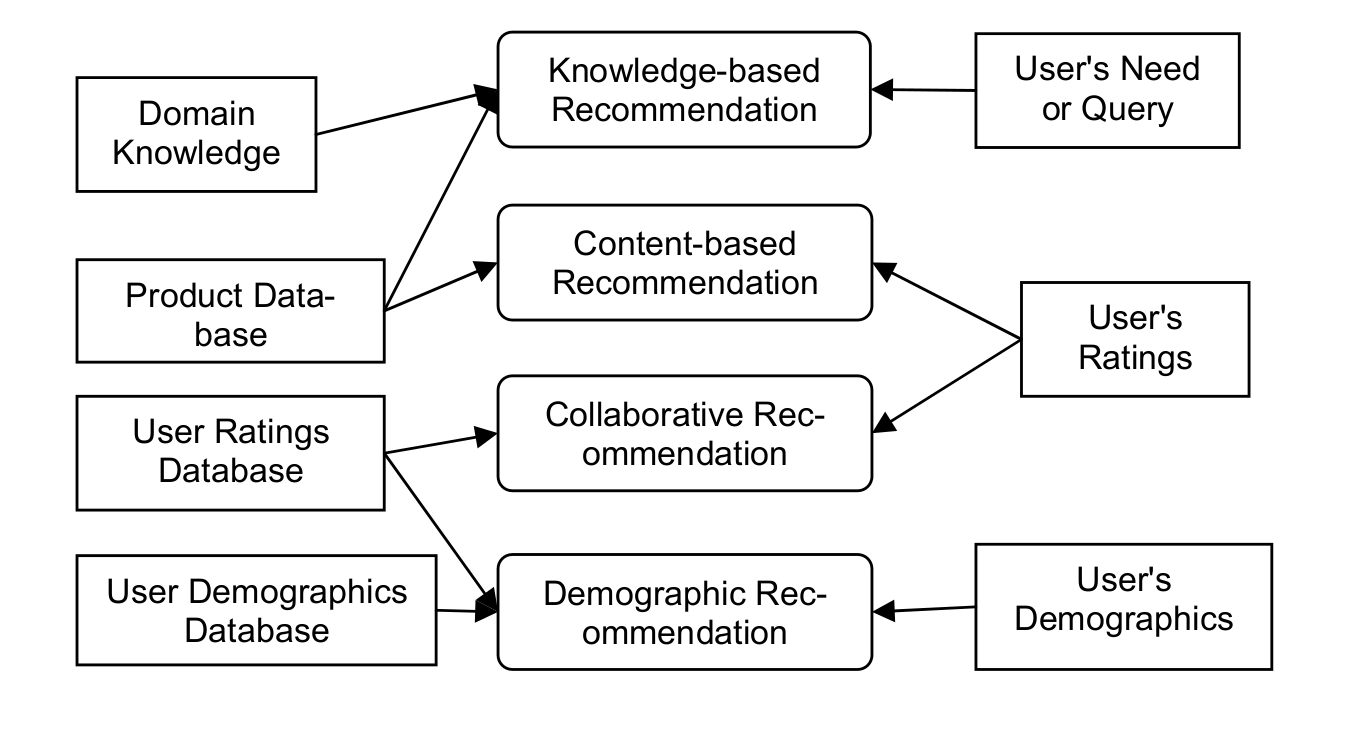
\includegraphics[scale=0.3]{inc/recommendersystems/RecommendationTechniquesAndKnowledgeSources.png}
    \caption{Recommendation techniques and their knowledge sources.\citep[p.~379]{burke:2007}}
\end{figure}

\subsection{Comparison}
%%%%%%%%%%%%%%%%%%%%%%%%%%%%%%%%%%%%
vor- und nachteile
\"Ubersicht \"uber alle System (fancy Tabelle?)
%%%%%%%%%%%%%%%%%%%%%%%%%%%%%%%%%%%%

\section{Mixing different RS approaches together}
%%%%%%%%%%%%%%%%%%%%%%%%%%%%%%%%%%%%
\iffalse
Hybrid web recommender systems
\fi
%%%%%%%%%%%%%%%%%%%%%%%%%%%%%%%%%%%%

\subsection{Critics on RS}
%%%%%%%%%%%%%%%%%%%%%%%%%%%%%%%%%%%%
Bei Onlinezeitungen: Nutzer bekommen nur noch Artikel die sie lesen wollen --> verdummung?
%%%%%%%%%%%%%%%%%%%%%%%%%%%%%%%%%%%%
